\subsection{Thread Spawner}

\begin{figure}[H]
	\centering
	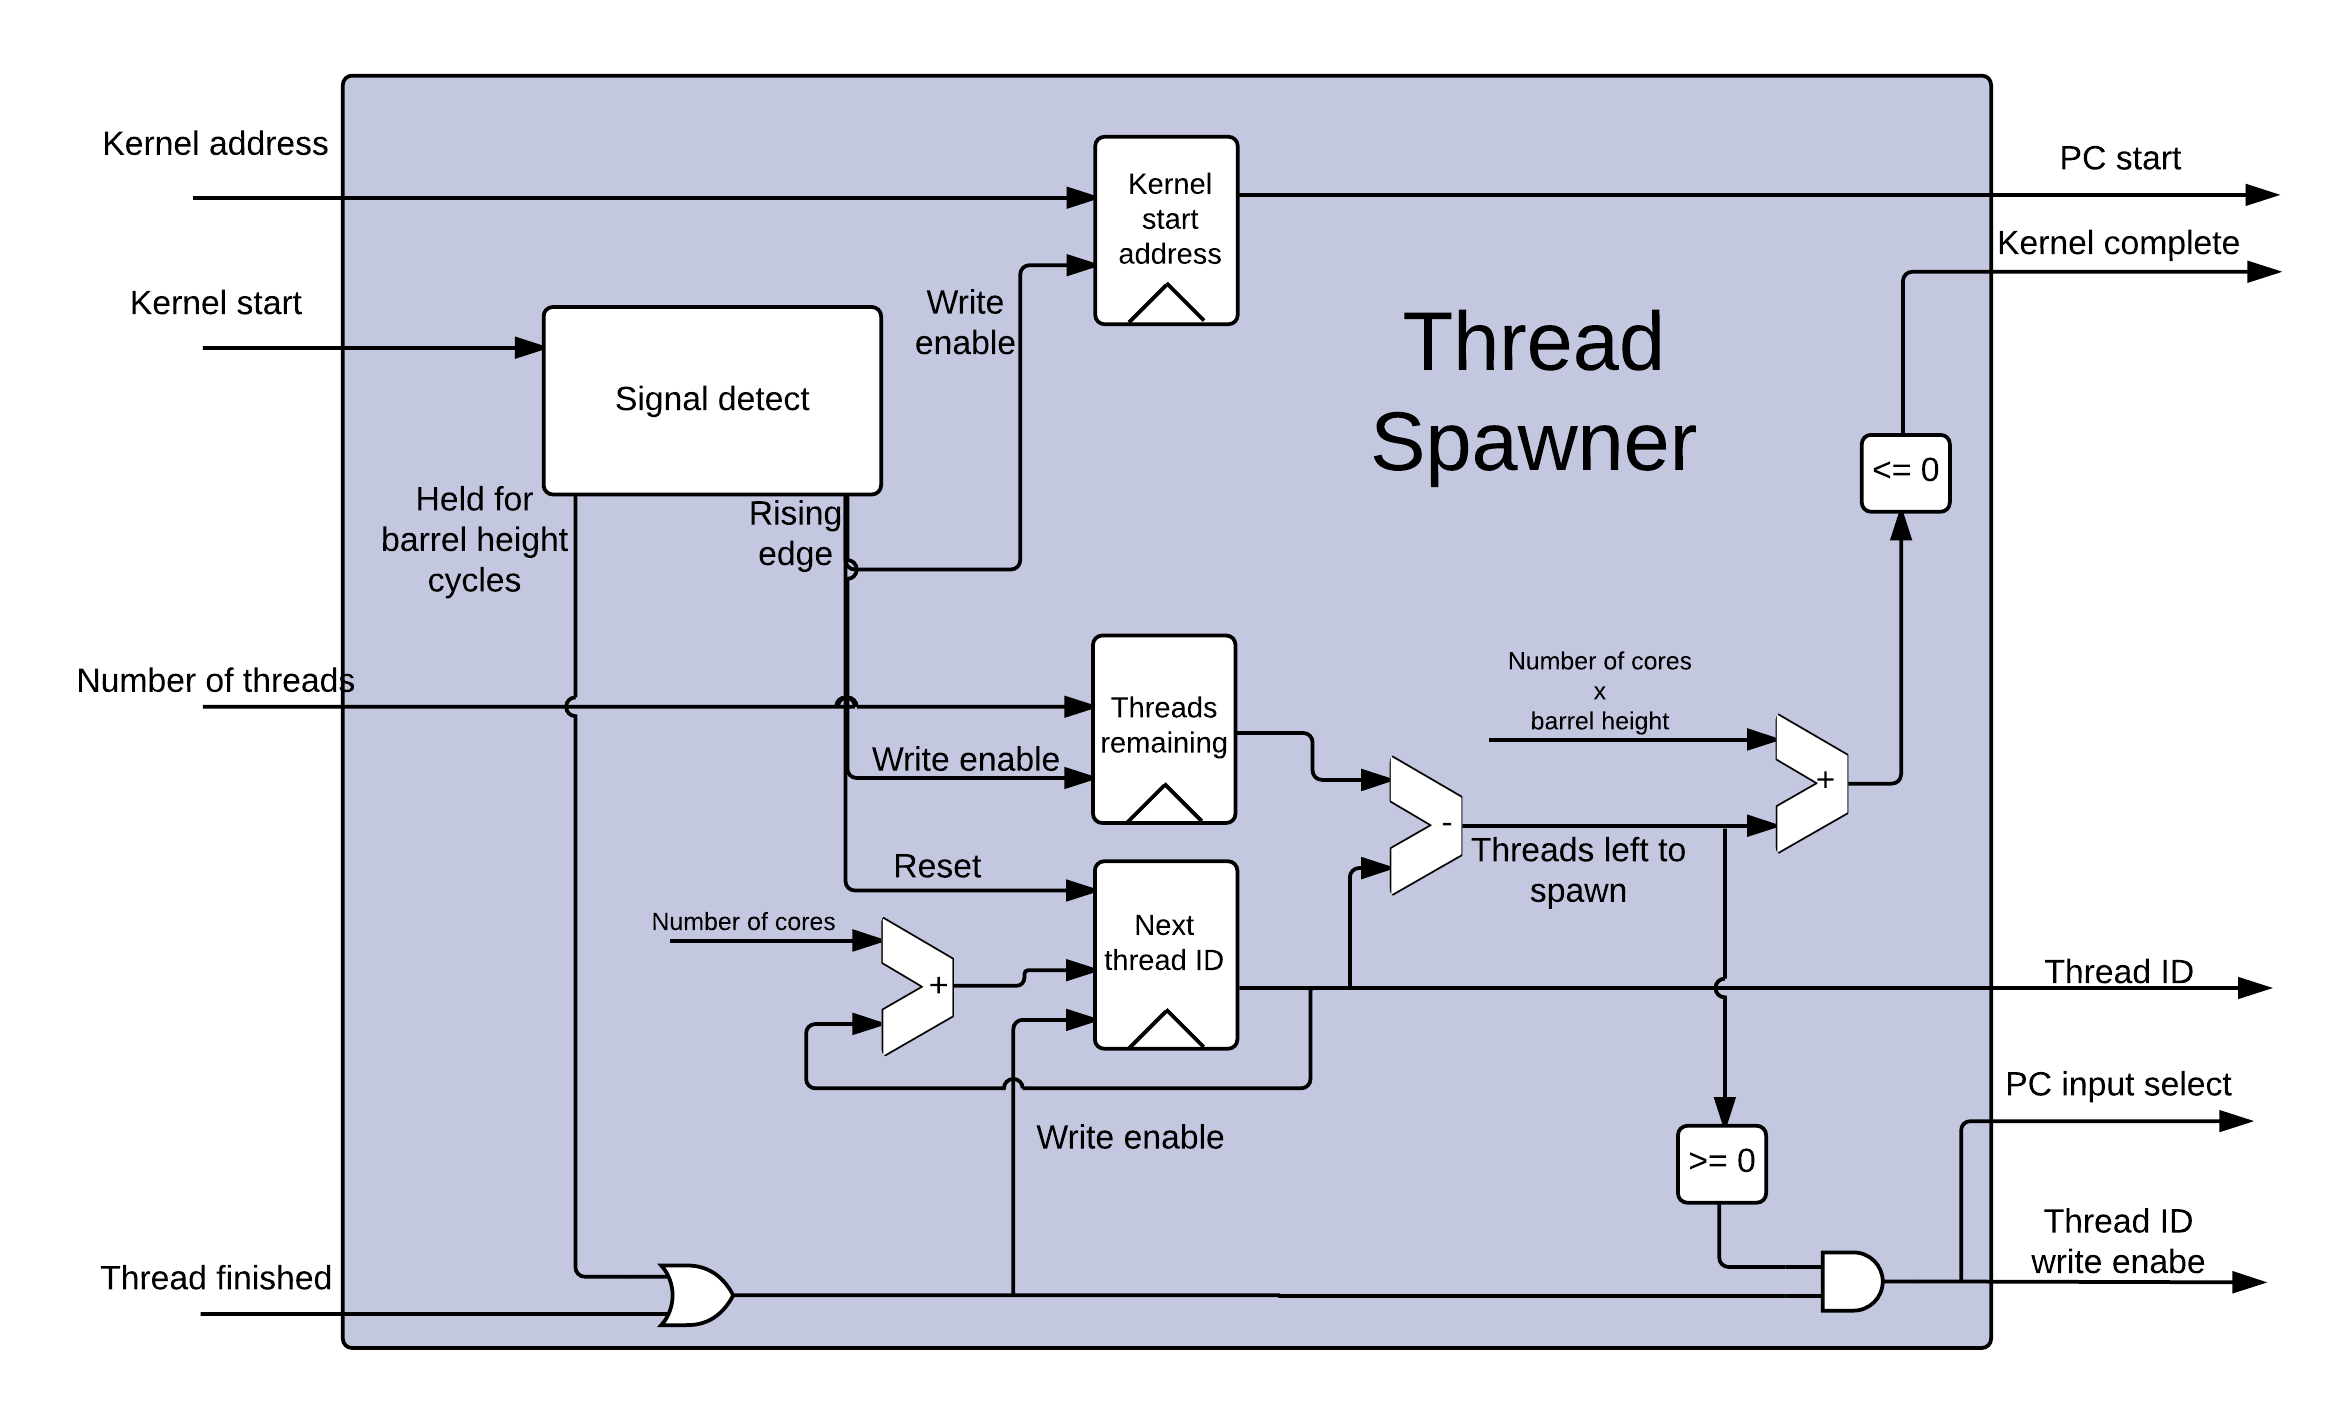
\includegraphics[width=\textwidth]{../gpu/diagrams/thread_spawner.png}
	\caption{Thread spawner and neighboring components}
	\label{fig:thread_spawner}
\end{figure}

The thread spawner is responsible for overseeing kernel execution.
It controls the program counter, spawns threads whenever necessary, and asserts the kernel done signal when execution has finished.

When a kernel invocation request is received, the thread spawner stores the provided base address of the kernel, the number of threads to spawn, and sets the next thread ID register to zero.
If the 'start kernel' or the 'finished' signal is asserted, and there are threads left to spawn (by comparing the number of threads to spawn with the next thread ID register) then a new warp of threads is spawned.

This is accomplished by writing the next thread ID to all ID registers in the currently active barrel line, incremented by the index of the target streaming processor.
The next thread ID is then incremented by the warp size.
If the warp is spawned into barrel line zero, the program counter will be reset to the kernel base address, and the first instruction of the kernel will start trickling down the barrel lines.
A new warp of threads has been spawned!
